\chapter{Project Loom}
\label{cha:ProjectLoom}

\section{Überblick}                                         % 1-2 Seiten
\label{sec:Überblick}

    Projekt Loom wurde 2017 von Ron Pressler ins Leben gerufen und ist ein Open-Source-Projekt, 
    das sich auf die Verbesserung der \gls{jvm} konzentriert. Das Ziel von Project Loom ist es, 
    die \gls{jvm} so zu erweitern, dass der Aufwand für das Schreiben, Warten und Überwachen von hochdurchsatzfähigen nebenläufigen Anwendungen,
    die die verfügbare Hardware optimal nutzen, drastisch reduziert wird.
    \cite{ProjectLoom}

    Die wichtigste Neuerung sind \textbf{\Glspl{vt}}.
    Virtuelle Threads sind Threads, die im Gegensatz zu \Glspl{pt} von der JVM verwaltet werden und nicht direkt vom Betriebssystem. 
    Sie sind leichtgewichtiger als normale Threads, da sie weniger Speicher benötigen und schneller erstellt werden können. \cite{JEP444}
    Virtuelle Threads sind auch als Continuations bekannt und werden in anderen Programmiersprachen wie Python, Ruby und JavaScript verwendet.
    Project Loom soll die JVM so erweitern, dass sie virtuelle Threads unterstützt und Entwicklern eine einfachere Möglichkeit bietet,
    nebenläufige Anwendungen zu erstellen. Virtuelle Threads sollen die Leistung von Java-Anwendungen verbessern, indem sie die Anzahl der Threads reduzieren und 
    die Verwaltung von Threads vereinfachen. 

    Aufbauend darauf wird auch \textbf{Strukturierte Nebenläufigkeit (Structured Concurrency)} vorgestellt.
    Diese sollen eine Gruppe von Threads die parallel ausgeführt werden aber verwandte Aufgaben erledigen, als eine eine Arbeitseinheit behandeln. 
    Dabei soll keine Sicherheit oder Kontrolle über die einzelnen Aufgaben eingebüßt werden sondern Kontrolle über das Gesamtverhalten der Gruppe gewonnen werden.
    Dies soll eine parallele Ausführung von verschiedenen Aufgaben einfacher gestalten und die Fehlersuche erleichtern.
    Im Hintergrund kommen dafür \Glspl{vt} zum Einsatz. \cite{JEP453}

    \textbf{Bereichsgebundene Werte (Scoped Values)} sind Werte deren Gültigkeitsbereich nach belieben festgelegt werden kann.
    Auch Verschachtelungen der Bereiche oder das
    Zuweisen verschiedener Werte auf verschiedenen Threads, ähnlich zu \texttt{ThreadLocal<>} sind möglich. Ihre Effizienz wurde auf \Glspl{vt} optimiert.
    \cite{JEP481}
    Project Loom ist ein laufendes Projekt und manche Funktionalitäten sind noch als Preview-Funktionalität eingestuft und können in späteren Versionen Änderungen 
    unterzogen werden oder sogar wieder entfernt werden.

    

\section{Virtuelle Threads}                                 % 5 Seiten ---------------------------------------------------------------------------------------------------------
\label{sec:VirtuelleThreads}


\subsection{Was sind Virtuelle Threads?}
\label{subsec:WassindVTs?}

    Im Gegensatz zu dem bisherigen Threadmodell von Java hängt die Implementierung von \Glspl{vt} nicht so stark von den \Glspl{ot} ab. Sie führen zwar noch Code 
    auf diesen aus aber binden diesen nicht mehr ihre gesamte Lebenszeit lang im Gegensatz zu den herkömmlichen \Glspl{pt}. Dies hat zur folge dass mehrere 
    \Glspl{vt} Aufgaben zeitversetzt auf ein und demselben \gls{ot} ausführen können und die maximale Anzahl der \Glspl{vt}
    die maximale Anzahl von \Glspl{ot} überschreiten kann.
    Virtuelle Threads werden aber nicht direkt auf OS Threads aufgesetzt sondern auf Plattform Threads daher werden diese auch oft als "Carrier Threads" bezeichnet.
    \cite{ieee2022}

    \begin{figure}[H]
        \centering
        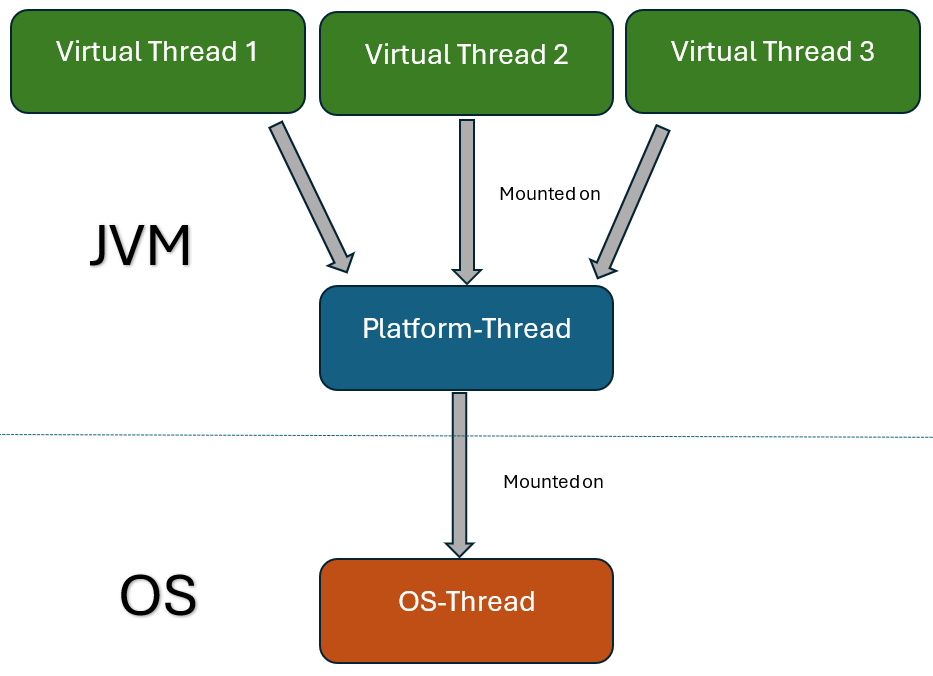
\includegraphics[width=0.6\textwidth]{VTs}
        \caption{Virtuelle Threads in der JVM}
        \label{fig:VTs}
    \end{figure}

    Da \Glspl{vt} vollkommen von der \gls{jvm} verwaltet werden und da diese über die Art von Aufgabe und derzeitigen Zustand des Threads Bescheid weiß kann die
    \gls{jvm} einen \gls{vt} von dem ihm zugeteilten \gls{pt} temporär lösen und einen anderen \gls{vt} darauf Code ausführen lassen da das Blockieren von \Glspl{vt}
    sehr billig ist. Dies hat zur Folge dass \Glspl{vt} nur dann Rechenzeit erhalten wenn sie auch benötigt wird. Somit wird der Durchsatz an Recheninstruktionen
    eines \gls{pt} stark erhöht.
    Wird aber nur ein einzelner Thread benötigt können diese Vorteile nicht genutzt werden. Der \gls{pt} dem der \gls{vt} zugewiesen wurde bindet den \gls{ot} auch an sich
    selbst wenn kein \gls{vt} Code ausführt.
    \cite{JEP444}

    \begin{figure}[H]
        \centering
        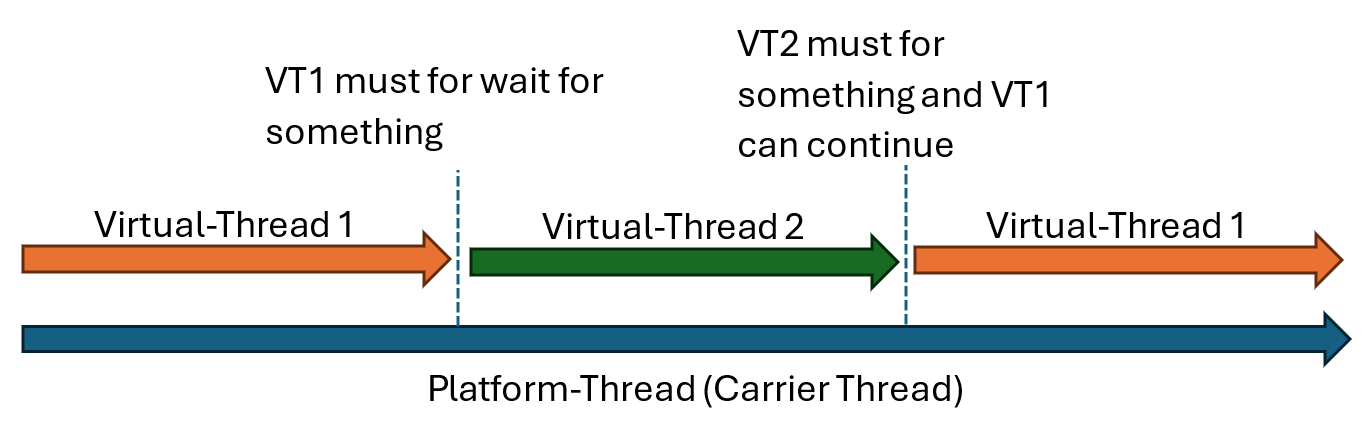
\includegraphics[width=0.67\textwidth]{VT_Coroutine}
        \caption{Coroutine von \Glspl{vt}}
        \label{fig:VT_Coroutine}
    \end{figure}

    Die \gls{jvm} kann auch die initiale Ressourcenzuweisung viel präziser durchführen und besitzt auch die Fähigkeit den Stapel während der Laufzeit dynamisch 
    schrumpfen zu lassen. Vor allem bei Anwendungen die viele Threads über einen längeren Zeitraum  laufen lassen kann trägt dies zur Effizienz und Stabilität bei.
    Ansonsten unterscheiden sich \Glspl{vt} nicht stark von \Glspl{pt} und werden von den gleichen Problemen geplagt wie z.B.: Deadlocks, Race Conditions
    \cite{JEP425}


\subsection{Wie werden VTs benutzt?}
\label{subsec:WieWerdenVTsBenutzt?}

    Die Erstellung und Verwendung von virtuellen Threads unterscheidet sich nicht stark von den platform Threads. 
    \begin{program} [H]
        \caption{Erstellung eines \Glspl{vt}}
        \label{prog:ErstellungEinesVT}
        % \begin{JavaCode}
    \begin{JavaCode}[language=Java, numbers=left]
public class VirtualThreadExample {
    public static void main(String[] args) {
        Thread vt = Thread.ofVirtual().name("VirtualThread").start(() -> {
            System.out.println("Hello from a virtual thread!");
        });
        vt.setPriority(Thread.MAX_PRIORITY);
        try {
            vt.join();
        } catch (InterruptedException e) {
            e.printStackTrace();
        }
    }
}
    \end{JavaCode}
    \end{program}
    Anstatt \texttt{new Thread(Runnable task).start();} wird der Ausdruck aus Zeile 3 in Programm 
    \ref{prog:ErstellungEinesVT} benutzt um einen neuen Thread zu erstellen und zu starten. \texttt{Thread.join();} lässt genauso wie bei \Glspl{pt} den aktuellen Thread 
    auf die Beendung des Threads warten für den \texttt{.join();} aufgerufen wurde. Die Nachteile dieser Art der Verwendung sind Codeduplizierung und erhöhter Aufwand
    beim Starten mehrerer Threads da Eigenschaften wie der Name für jeden Thread individuell angepasst werden müssen.
    Weiters besteht auch die Möglichkeit einen Thread.Builder zu benutzen der die Anpassung solcher Eigenschaften wie eine Zeichenkette und fortlaufende Zahl
    als Name selbständig weiterführt.
    \texttt{.setPriority(int);} verändert aber nur die Priorität des \Glspl{vt} und nicht die des zugrundeliegenden \Glspl{pt}. Dadurch ist die Wirkung des Ausdruckes
    stark eingeschränkt.
    
    \begin{program} [H]
        \caption{Example of a virtual threadbuilder in Java}
        \label{prog:ErstellungEinesVTBuilders}
    \begin{JavaCode}[language=Java, numbers=left]
public class VirtualThreadBuilderExample throws InterruptedException{
    public static void main(String[] args) {
        Thread.Builder builder = Thread.ofVirtual().name("worker-", 0);
        Runnable task = () -> {
            // do something
        };
        // name "worker-0"
        Thread t1 = builder.start(task);
        t1.setPriority(Thread.MAX_PRIORITY);   
        t1.join();
        System.out.println(t1.getName() + " terminated");
        // name "worker-1"
        Thread t2 = builder.start(task);   
        t2.join();  
        System.out.println(t2.getName() + " terminated");

        try {
            t1.join(); t2.join();
        } catch (InterruptedException e) {
            e.printStackTrace();
        }
    }
}
    \end{JavaCode}
    \end{program}

    Dabei können Regeln für verschiedene Attribute wie eine Namenskonvention wie in Zeile 3 in \ref{prog:ErstellungEinesVTBuilders}
    in einem Schritt für alle späteren Threads festgelegt werden was Codeduplizierung entgegenwirkt.

    \begin{program} [H]
        \caption{Example of a virtual threadbuilder in Java}
        \label{prog:ErstellungEinesExecutors}
    \begin{JavaCode}[language=Java, numbers=left]
public class VirtualThreadExecutorExample {
    public static void main(String[] args) {
        try (var executor = Executors.newVirtualThreadPerTaskExecutor()){
            IntStream.range(0, 1000).forEach(i -> {
                executor.execute(() -> {     //.submit() returns a Future<> object that can be used to retrieve the result of a computation; .execute() does not return a result.
                    System.out.println("Thread " + i + " started");
                });
            });
        }       // executor.close() is called is called implicitly and the Thread waits for all tasks to finish
        System.out.println("All Tasks finished"); 
    }
}
    \end{JavaCode}
    \end{program}

    Wird eine große Anzahl an \Glspl{vt} benötigt  ist ein Executor bzw. Threadpool empfehlenswert. Dieser sollte in Kombination mit einem
    try-with-resources-Block verwendet werden da dieser beim Verlassen des Blockes implizit geschlossen wird. Der .newVirtualThreadPerTaskExecutor();
    erstellt im Gegensatz zum \texttt{.newFixedThreadPool();} für jede Aufgabe einen neuen \gls{vt}.
    Sollten die Aufgaben einen Wert retournieren muss anstatt .execute(); .submit(); benutzt werden. Dies retourniert ein Future<T>-Objekt. Der Wert kann mit der
    .get() - Methode ausgelesen werden die auch darauf wartet dass der Wert auch schon zugewiesen wurde.
    \cite{oracle21VritualThreads}


\section{Structured Concurrency}                                 % 4 Seiten ---------------------------------------------------------------------------------------------------------
\label{sec:Structured Concurrency}


\subsection{Was ist Structured Concurrency?}
\label{subsec:WasistSC?}
    Der Bereich Strukturierte Nebenläufigkeit (Structured Concurrency) in project Loom fügt \Glspl{sts} hinzu und befindet sich derzeit noch in
    aktiver Entwicklung. Das heißt dass sich verschieden Funktionalitäten ändern oder wieder entfernt werden können.
    Die zu Strukturierte Nebenläufigkeit gehörigen Klassen ermöglichen
    es eine Gruppe von parallelen Teilaufgaben als eine Einheit zu Koordinieren. Allgemeine Ausführungslogik und Fehlerbehandlung kann dadurch schon vorher festgelegt und 
    wiederverwendet werden.
    Wie der Name bereits verrät wird dabei ein Block festgelegt in dem diese Teilaufgaben erstellt und behandelt werden.
    Dadurch müssen die Teilaufgaben vor dem Hauptprozess in dem sie gestartet wurden beendet werden.
    \cite{oracle21SC}

    \begin{program} [H]
        \caption{Beispiel für einen einfachen \gls{sts}}
        \label{prog:BeispielFürEinenEinfachenSts}
    \begin{JavaCode}[language=Java, numbers=left]
public class StructuredTaskScopeExample {
    public static void main(String[] args) {
        try (var scope = new StructuredTaskScope<>()) {
            StructuredTaskScope.Subtask<String> result1 = scope.fork(() -> {
                Thread.sleep(1000);
                return "Result from task 1";
            });
            var result2 = scope.fork(() -> {
                Thread.sleep(2000);
                throw new RuntimeException("Task 2 failed");
            });
            StructuredTaskScope.Subtask<Integer> result3 = scope.fork(() -> {
                Thread.sleep(3000);
                return 3;
            });
            scope.join();                        // Waits for all subtasks to complete
            System.out.println(result1.get());
            System.out.println(result2.get());   // Throws an ExecutionException
            System.out.println(result3.get());   // Throws an ExecutionException because the second task failed
        } catch (Exception e) {                 // calls .close() implizit.
            e.printStackTrace();
        }
    }
}
    \end{JavaCode}
    \end{program}
    Es wird stark empfohlen einen \gls{sts} in Form eines try-with-resources-Blocks zu realisieren da dieser den Gültigkeitsbereich wieder schließt. In diesem Block
    werden Teilaufgaben mit der Methode \texttt{.fork(Runnable r);} erschaffen. Diese haben den Rückgabewert \texttt{StructuredTaskScope.Subtask<T>} wobei sie keine
    atomaren Datentypen aufnehmen können. Mit \texttt{.state();} kann überprüft werden ob die Ausführung erfolgreich war.
    Wichtig dabei ist der Aufruf von \texttt{.join();}. Dadurch wartet der \gls{sts} darauf dass entweder alle Teilprozesse beendet werden oder fehlschlagen oder
    eine andere vordefinierte Abbruchbedingung erreicht wird.
    \cite{oracle21STS}

    \begin{program} [H]
        \caption{Beispiel für ShutdownOnFailure}
        \label{prog:BeispielFürShutdownOnFailure}
    \begin{JavaCode}[language=Java, numbers=left]
public class ShutdownOnFailureExample {
    public static void main(String[] args) {
        System.out.println("Shutting down on failure ...");
        StructuredTaskScope.Subtask<String> result1 = null;
        StructuredTaskScope.Subtask<String> result2 = null;
        StructuredTaskScope.Subtask<String> result3 = null;
        try (var scope = new StructuredTaskScope.ShutdownOnFailure()) {            // shuts down the scope if a subtask fails
            result1 = scope.fork(() -> {
                Thread.sleep(1000);
                return "Result from task 1";
            });
            result2 = scope.fork(() -> {                                           // used to return a Future<> object
                Thread.sleep(2000);
                throw new RuntimeException("Task 2 failed");
            });
            result3 = scope.fork(() -> {
                Thread.sleep(5000);
                return "Result from task 3";
            });
            scope.join().throwIfFailed();
            if (result1.state() == StructuredTaskScope.Subtask.State.SUCCESS) {
                System.out.println("Task 1 completed");
            }
        } catch (Exception e) {
            System.out.println("Scope failed");
        }
        System.out.println(result1.get());                                          
        System.out.println(result2.get());
        System.out.println(result3.get());                      // Throws an IllegalStateException if the scope is shut down due to the exception in the second task
    }
}
    \end{JavaCode}
    \end{program}
    


